\documentclass{beamer}
\usepackage{parskip}
\usepackage{graphicx}
\usepackage{amsmath}
\usepackage{tikz}
\usepackage{float}
\usepackage[swedish,english]{babel}
\usepackage{amsmath}
\usepackage{amssymb}
\usepackage{color}
\usepackage{lipsum}
\usepackage{subcaption}
\usepackage[font={small}]{caption}
\usepackage{booktabs}
\usepackage{tikz}
\usetikzlibrary{decorations, matrix, arrows, shapes, positioning, calc, fit}
\tikzset{
   mybox/.style={draw, minimum height=.6cm, minimum width=.5cm},
   myflip/.style={draw, fill=gray!30, minimum height=.6cm, minimum width=.5cm},
   myint/.style={draw, minimum height=.7cm, minimum width=1cm},
   mynone/.style={draw=none}
}
\usepackage{graphicx,epstopdf}
\epstopdfsetup{update} % only regenerate pdf files when eps file is newer
\usepackage{cleveref}
\usepackage{collcell} % loads array
\newcolumntype{m}{>{$} r <{$}}
\newcolumntype{u}{>{$[\collectcell\si} l <{\endcollectcell]$}}
\newcommand{\approxtext}[1]{\ensuremath{\stackrel{\text{#1}}{=}}}
\newcommand{\matr}[1]{\mathbf{#1}}
\newcommand{\partt}[2]{\ensuremath{\dfrac{\partial {#1}}{\partial {#2}}}}
\renewcommand{\d}[1]{\ensuremath{\operatorname{d}\!{#1}}} % non-italized differentials
\newcommand{\h}[0]{\ensuremath{\hbar}} % hbar
\def\changemargin#1#2{\list{}{\rightmargin#2\leftmargin#1}\item[]}
\let\endchangemargin=\endlist 
\usepackage{amsthm}
\theoremstyle{plain}
\newtheorem{thm}{theorem} % reset theorem numbering for each chapter
\theoremstyle{definition}
\newtheorem{defn}[thm]{definition} % definition numbers are dependent on theorem numbers
\newtheorem{exmp}[thm]{example} % same for example numbers
\renewcommand{\theequation}{\thesection.\arabic{equation}}
\def\changemargin#1#2{\list{}{\rightmargin#2\leftmargin#1}\item[]}
\let\endchangemargin=\endlist    
\newcommand{\ts}{\textsuperscript} 
\usepackage[log-declarations=false]{xparse}
\usepackage{epstopdf}

\usetheme{metropolis}

\graphicspath{{figures/}}

\title
{
   Linking the Dynamics of Genetic Algorithms \\
   to the Encoding of Information
}
\date{\today}
\author
{
   Henrik \r{A}hl\\
   \small{Supervised by Carl Troein and Adriaan Merlevede}
}

\begin{document}
\begin{frame}
	\titlepage
\end{frame}

\begin{frame}
\frametitle{Presentation overview}
\tableofcontents{}
\end{frame}


%\AtBeginSection[]
%{
%   \begin{frame}
%      \frametitle{Presentation overview}
%      \tableofcontents[currentsection,sectionstyle=show/shaded]
%   \end{frame}
%}
\section{An introduction to genetic algorithms}

\begin{frame}
	\frametitle{Algorithms inspired by evolution}
      Genetic algorithms evolve \textit{data sequences} by using the concepts of
      \textit{mutation}, \textit{reproduction} and \textit{selection}

      ...~for optimisation purposes
      
      ...~for solving hard combinatorial problems

      ...~for studying evolutionary dynamics

\end{frame}

\begin{frame}
	\frametitle{General structure}
   \begin{itemize}
      \item Genetic algorithms maintain a pool of \textit{candidate solutions} and
      modify them using \textit{mutation} and \textit{crossover} (recombination)
      operators

      \item A \textit{selection} operator determines which solutions are mutated,
      recombined or picked for survival\\[3em]
   \end{itemize}
\begin{figure}[H]
      \centering
      % Define tikz specific styles
      \tikzstyle{block} = [rectangle, draw, fill=white!20, 
          text width=5em, text centered, rounded corners, minimum height=3.5em]
      \tikzstyle{line} = [draw, -latex'] 
      \tikzstyle{cloud} = [draw,
         ellipse,fill=gray!30, node distance=3.5cm,
      minimum height=2.5em]
          
      \begin{tikzpicture}[->,>=stealth',auto, node distance=3cm, 
          thick,node/.style={box, draw,font=\sffamily\Large\bfseries},scale=.8,every node/.style={scale=.8}]

          % Place nodes
          \node [cloud] (init) {\begin{tabular}[H]{c}Initialization\\of population\end{tabular}};
          \node [block, right of=init, node distance=4cm] (mut) {Mutation};
          \node [block, right of=mut] (crossover) {Crossover};
          \node [block, right of=crossover] (selection) {Selection};
          \node [cloud, below of=crossover, node distance=1.7cm] (newp) {New population};

          % Draw edges
          \path [line] (init) -- (mut);
          \path [line] (mut) -- (crossover);
          \path [line] (crossover) -- (selection);
          \path [line] (selection) |- (newp);
          \path [line] (newp) -| (mut);
      \end{tikzpicture}
   \end{figure}
\end{frame}

\begin{frame}
	\frametitle{General structure}
  \begin{itemize}
   \item Information~(\textit{phenotype}) is encoded as a data sequence~(\textit{genotype})

   \item Phenotypes are evaluated by a \textit{fitness}, \textit{cost} or
   \textit{objective function}\\[3em]
\end{itemize}
   \begin{figure}[H]
      \centering
      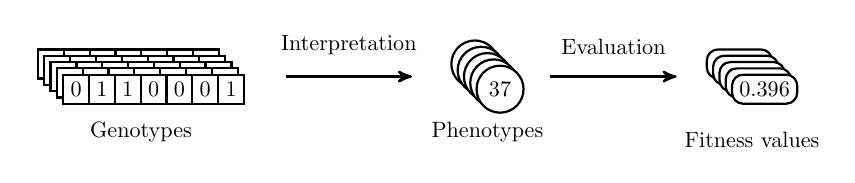
\begin{tikzpicture}[->,>=stealth',auto,
            thick,node/.style={box,
         draw,font=\sffamily\Large\bfseries},ampersand replacement=\&,scale=.8,
      every node/.style={scale=.8}]
            \matrix (matrix) at (-10.0,-.0)[
                matrix of nodes,
                column sep=-\pgflinewidth,
                row sep=-\pgflinewidth,
               row 1/.style={every node/.append style={draw,fill=white,minimum width=.5em, minimum height=.4em}},
            ]{
              0  \& 1\&  1 \& 0 \& 0 \& 0 \& 1   \\
            };
            \matrix (matrix2) at (-9.9,-.1)[
                matrix of nodes,
                column sep=-\pgflinewidth,
                row sep=-\pgflinewidth,
                row 1/.style={every node/.append style={draw,fill=white,minimum width=.5em, minimum height=.4em}},
            ]{
              0 \& 1 \& 1 \& 0 \& 0 \& 0 \& 1   \\
            };
            \matrix (matrix3) at (-9.8,-.2)[
                matrix of nodes,
                column sep=-\pgflinewidth,
                row sep=-\pgflinewidth,
                row 1/.style={every node/.append style={draw,fill=white,minimum width=.5em, minimum height=.4em}},
            ]{
              0 \& 1 \&  1 \& 0 \& 0 \& 0 \& 1   \\
            };
            \matrix (matrix4) at (-9.7,-.3)[
                matrix of nodes,
                column sep=-\pgflinewidth,
                row sep=-\pgflinewidth,
                row 1/.style={every node/.append style={draw,fill=white,minimum width=.5em, minimum height=.4em}},
            ]{
              0 \& 1 \& 1 \& 0 \& 0 \& 0 \& 1   \\
            };
            \matrix (matrix5) at (-9.6,-.4)[
                matrix of nodes,
                column sep=-\pgflinewidth,
                row sep=-\pgflinewidth,
                row 1/.style={every node/.append style={draw,fill=white,minimum
                width=.5em, minimum height=.4em,anchor=south}},
            ]{
              0 \& 1 \& 1 \& 0 \& 0 \& 0 \& 1   \\
            };

            \node [fill=none, below of=matrix3, node distance=2.5em] (init) {Genotypes};

             \tikzstyle{circ} = [draw, circle,fill=white!100, node distance=3cm,minimum height=1.5em]
             
             \node  [circ] at (-4.5,-.0) (1) {37};
             \node  [circ] at (-4.4,-.1) (2) {37};
             \node  [circ] at (-4.3,-.2) (3) {37};
             \node  [circ] at (-4.2,-.3) (4) {37};
             \node  [circ] at (-4.1,-.4) (5) {37};
             
             \node [fill=none, below of=3, node distance=2.5em] (pheno) {Phenotypes};
             
             \node  [rectangle, draw,fill=white!100, rounded corners] at (-.30,-.0) (11) (fitness1) {0.396};
             \node  [rectangle, draw,fill=white!100, rounded corners] at (-.20,-.1) (21) (fitness2) {0.396};
             \node  [rectangle, draw,fill=white!100, rounded corners] at (-.10,-.2) (31) (fitness3) {0.396};
             \node  [rectangle, draw,fill=white!100, rounded corners] at (-.00,-.3) (41) (fitness4) {0.396};
             \node  [rectangle, draw,fill=white!100, rounded corners] at (+.10,-.4) (51) (fitness5) {0.396};

             \node  [fill=none, below of=fitness3] (fit) {Fitness values};
             \tikzstyle{line} = [draw, -latex']
             \draw [->] (-7.5,-.2)-- (-5.5,-.2){};
             \draw [->] (-7.5,-.2)--(-5.5,-.2) node [midway, above=.5em] (interpret) {Interpretation};
             
             \draw [->] (-3.3,-.2)--(-1.3,-.2){};
             \draw [->] (-3.3,-.2)--(-1.3,-.2) node [midway, above=.5em ] (eval) {Evaluation};
         \end{tikzpicture}
   \end{figure}
\end{frame}

\begin{frame}
	\frametitle{The search space}
   \begin{itemize}
      \item The algorithms traverse a \textit{fitness
         landscape}, or \textit{search space}   
   \end{itemize}
   \begin{figure}[H]
      \centering
      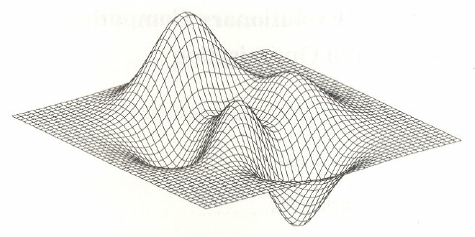
\includegraphics[width=.6\textwidth]{landscape}
   \end{figure}
   \begin{itemize}
      \item This is done by mutating and recombining the current data structures
         to produce new sample points
   \end{itemize}
\end{frame}

\begin{frame}
	\frametitle{Genetic operators}
   \begin{itemize}
      \item The  \textbf{mutation} operator changes the genome such that a new candidate
         solution is produced\\[.8em]
      A common choice is the \textit{point mutation} operator
   \end{itemize}

   \begin{figure}[H]
      \centering
      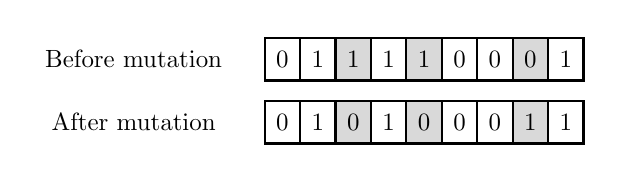
\begin{tikzpicture}[->,>=stealth',auto,scale=.9,
     thick,node/.style={box, draw,font=\sffamily\Large\bfseries}, every
  node/.style={scale=.9,anchor=south}]
      \matrix (matrix) [
          matrix of nodes,
          row sep={.8cm,between origins}, column sep=-\pgflinewidth,
          row 1/.style={every node/.append style={mybox}},
          row 2/.style={every node/.append style={mybox}},
          ampersand replacement=\&
      ]{
        |[draw=none]| Before mutation\hspace{.5cm} \&  0 \& 1 \& |[myflip]| 1 \& 1 \& |[myflip]| 1 \& 0 \& 0 \& |[myflip]| 0 \& 1   \\
        |[draw=none]| After mutation\hspace{.5cm}  \&  0 \& 1 \& |[myflip]| 0 \& 1 \& |[myflip]| 0 \& 0 \& 0 \& |[myflip]| 1 \& 1   \\
      };
      \end{tikzpicture}
\end{figure}

   \begin{itemize}
      \item The \textbf{selection} operator determines diversity and bias by picking
         individuals for survival or reproduction\\[.8em]
         A common choice is
         \textit{tournament selection}
   \end{itemize}

\end{frame}

\begin{frame}
	\frametitle{The encoding and decoding is problem specific}
   \begin{figure}[H]
      \centering
      \begin{tikzpicture}[->,>=stealth',auto,
            thick,node/.style={box, draw,font=\sffamily\Large\bfseries},ampersand replacement=\&,scale=.8, every node/.style={scale=.8}]
            \matrix (matrix) at (-10.0,-.0)[
                matrix of nodes,
                column sep=-\pgflinewidth,
                row sep=-\pgflinewidth,
               row 1/.style={every node/.append style={draw,fill=white,minimum
               width=1.5em, minimum height=1.4em,anchor=south}}
            ]{
              1 \& 1 \& 0 \& 1\&  1 \& 0 \& 0 \& 0 \& 1   \\
            };

             \tikzstyle{circ} = [draw, circle,fill=white!100, node distance=3cm,minimum height=1.5em]
             
             \node  [circ, right of=matrix, node distance=6cm]  (number_phenotype) {37};

            \matrix (matrix2) [below of=matrix,node distance=2cm,
                matrix of nodes,
                column sep=-\pgflinewidth,
                row sep=-\pgflinewidth,
               row 1/.style={every node/.append style={draw,fill=white,minimum
               width=1.5em, minimum height=1.4em, anchor=south}}
            ]{
            1.1 \& 1.4 \& 0.4 \& 1.9\&  6.1 \& 5.1 \& 2.2 \& 0.0 \& 1.0   \\
            };

             \node  [below of=number_phenotype, node distance=2cm]  (wings)
             {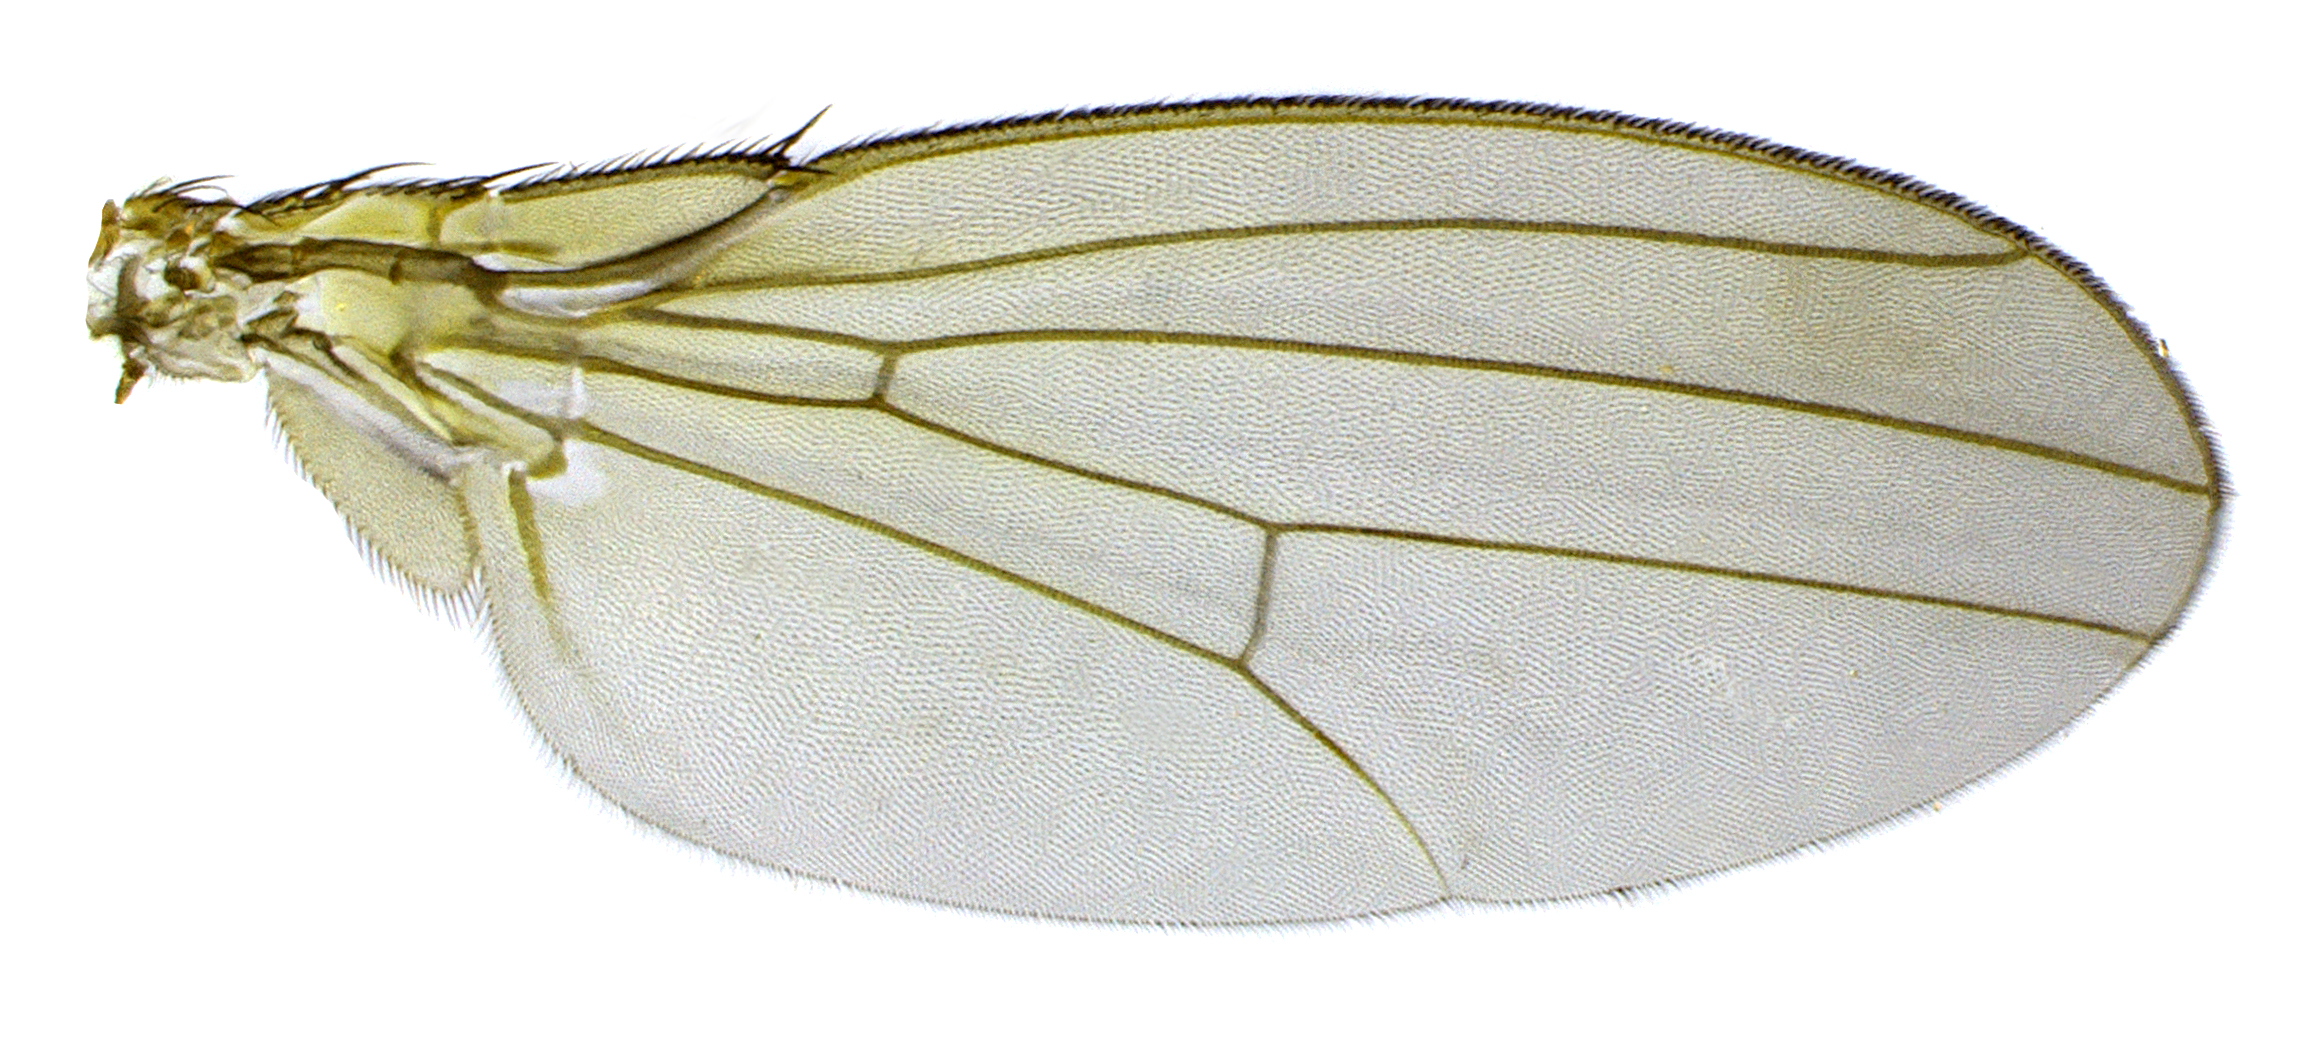
\includegraphics[width=.25\textwidth]{wings}};

             \matrix (matrix3) [below of=matrix2,node distance=2.3cm,
                matrix of nodes,anchor=center,
                column sep=-\pgflinewidth,
                row sep=-\pgflinewidth,
               row 1/.style={every node/.append style={draw,fill=white,minimum
               width=1em, minimum height=1.3em, anchor=south}},
            ]{
            \texttt{true} \&  \texttt{false} \& \texttt{false}  \& \texttt{false}\& \texttt{false}  \\
            };

            \tikzstyle{circ} = [draw, circle,fill=white!100, node distance=1.5cm,minimum height=1.5em]
            \node[circ, below of=wings] (A){};
            \node[circ, below of=A, left of=A] (B){};
            \node[circ, below of=A, right of=A] (C){};
            \node[fit=(A)(B)(C), right of=matrix3] (net){};
         \node[fill=white!100,below of=matrix3, node distance=2cm] (gen) {Genotypes};
         \node[fill=white!100,right of=gen, node distance =6cm] (phen) {Phenotypes}; 
            \path[every node/.style={font=\sffamily\small}]
            (B) edge[bend right] node[left] {}  (C)
            (C) edge[bend right] node[left] {}  (A)
            (A) edge[bend right] node[left] {}  (B)
            (C) edge[bend right] node[left] {}  (B)
            (B) edge [loop left] (B);
         \end{tikzpicture}
   \end{figure}
   Question: What are the differences between encodings which code for the same
   phenotype?
\end{frame}

\begin{frame}
	\frametitle{Encoding integers}
   Integers are normally encoded with a \textbf{Binary} encoding scheme
   \begin{figure}[H]
      \centering
      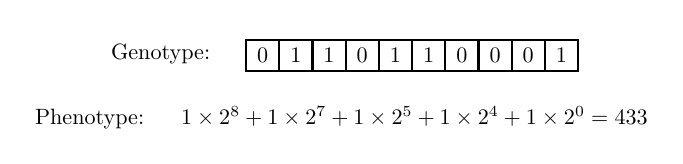
\begin{tikzpicture}[->,>=stealth',auto,
            thick,node/.style={box,
         draw,font=\sffamily\Large\bfseries},ampersand replacement=\&,scale=.8, 
         every node/.style={scale=.8}]
            \matrix (matrix) at (-10.0,-.0)[
                matrix of nodes,
                column sep=-\pgflinewidth,
                row sep=-\pgflinewidth,
               row 1/.style={every node/.append style={draw,fill=white,minimum
               width=1.5em, minimum height=1.4em,anchor=south}}
            ]{
            |[draw=none,fill=white!100]|Genotype:\ \ \ \ \  \&0 \& 1 \& 1 \& 0 \& 1\&  1 \& 0 \& 0 \& 0 \& 1   \\
            };
            \node [below of=matrix] (text) {Phenotype:\ \ \ \ \ $1\times 2^8 +1\times 2^7
               + 1\times 2^5 + 1\times 2^4 + 1\times 2^0 = 433$};
         \end{tikzpicture}
   \end{figure}
   Problem: adjacent phenotypes are not adjacent genotypes 
   (e.g.\ \texttt{0111} [7] and \texttt{1000} [8])

   Solution: \textbf{Gray code} -- all adjacent phenotypes are also adjacent
   genotypes
\end{frame}

\section{Experiment setup}
   \begin{frame}
      \frametitle{Algorithm settings}
         \begin{itemize}
            \item Population of 40 bitstrings
            \item All bitstrings are duplicated every generation
            \item Duplicates undergo point mutation ($p= 1 / \text{genome
               length}$)
            \item 40 new bitstrings are selected for survival by tournament
               selection
            \item No crossover operator 
         \end{itemize}
   \end{frame}

   \begin{frame}
      \frametitle{Algorithm objective}
         \begin{itemize}
         \item Find a set of 10 random integers, $I_i \in \left[ 
         0,1023\right]$
         \item The cost is measured as the sum of pairwise differences
         \end{itemize}

   \begin{figure}[H]
      \centering
      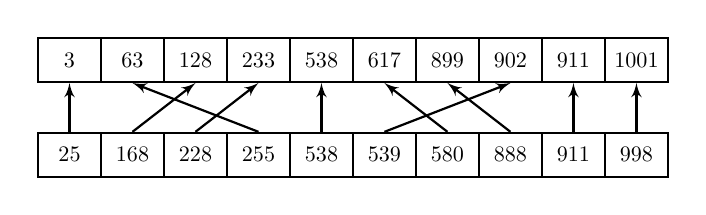
\begin{tikzpicture}[->,>=stealth',auto,
        thick,node/.style={box, draw,font=\sffamily\Large\bfseries},scale=.8,every node/.style={scale=.8, minimum height=1em}]
         \tikzstyle{line} = [draw, -latex']
            \matrix (matrix) 
            [
                matrix of nodes,
                row sep={.5cm,between origins}, column sep=-\pgflinewidth,
                row 1/.style={every node/.append style={myint}},
                row 2/.style={every node/.append style={myint}},
                ampersand replacement=\&
            ]
            {
               3  \& 63  \& 128 \& 233 \& 538 \& 617 \& 899 \& 902 \& 911 \& 1001 \\[2em]
               25 \& 168 \& 228 \& 255 \& 538 \& 539 \& 580 \& 888 \& 911 \& 998  \\
            };
            \path [line] (matrix-2-1.north) --  (matrix-1-1.south);
            \path [line] (matrix-2-2.north) --  (matrix-1-3.south);
            \path [line] (matrix-2-3.north) --  (matrix-1-4.south);
            \path [line] (matrix-2-4.north) --  (matrix-1-2.south);
            \path [line] (matrix-2-5.north) --  (matrix-1-5.south);
            \path [line] (matrix-2-6.north) --  (matrix-1-8.south);
            \path [line] (matrix-2-7.north) --  (matrix-1-6.south);
            \path [line] (matrix-2-8.north) --  (matrix-1-7.south);
            \path [line] (matrix-2-9.north) --  (matrix-1-9.south);
            \path [line] (matrix-2-10.north) -- (matrix-1-10.south);
      \end{tikzpicture}
   \end{figure}
         \begin{itemize}
         \item Smallest pairs are prioritised
         \end{itemize}
\end{frame}
   
   \begin{frame}
      \frametitle{Encodings used}
         \begin{itemize}
            \item Binary
            \item Gray code
            \item \textit{Consensus encodings}: ``Dead code'' with coding
               segments
         \end{itemize}
   \begin{figure}[H]
      \centering
      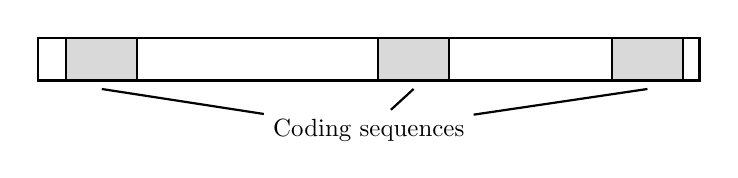
\begin{tikzpicture}[->,>=stealth',auto,scale=.9,
         thick,node/.style={box, draw,font=\sffamily\Large\bfseries}, every
         node/.style={scale=.9,anchor=south}]
      \matrix (matrix) [
          matrix of nodes,
          row sep={.8cm,between origins}, column sep=-\pgflinewidth,
          row 1/.style={every node/.append style={mybox}},
          row 2/.style={every node/.append style={mybox}},
          ampersand replacement=\&
      ]{
      |[style=draw,minimum width=.4cm]| \& |[style=draw,fill=gray!30,minimum
      width=1cm]| \&|[style=draw,minimum width=3.4cm]| \& |[style=draw,fill=gray!30,minimum
      width=1cm]| \& |[style=draw,minimum width=2.3cm]| \& |[style=draw,fill=gray!30,minimum
      width=1cm]| \& |[style=draw,minimum width=.2cm]|   \\
      };
      \node[below of=matrix] (test) {Coding sequences};
      \draw[-] (test)-- ([yshift=-3pt] matrix-1-2.south);
      \draw[-] (test)-- ([yshift=-3pt] matrix-1-4.south);
      \draw[-] (test)-- ([yshift=-3pt] matrix-1-6.south);
      \end{tikzpicture}
   \end{figure}

   \begin{itemize}
      \item Coding parts are signified by a start sequence of six bits:
         \texttt{110011}
   \end{itemize}
\end{frame}
\begin{frame}
   \frametitle{Search spaces}
   \vspace{1cm}
   \begin{figure}
      \centering
      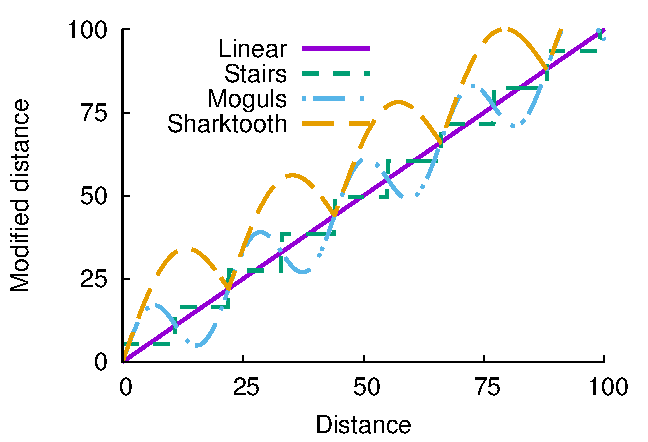
\includegraphics[width=.8\textwidth]{complexities-eps-converted-to}
   \end{figure}
\end{frame}

\section{Results}
   
\begin{frame}
   \frametitle{Performance}
   \vspace{2.5cm}
   \begin{figure}[H]
      \centering
      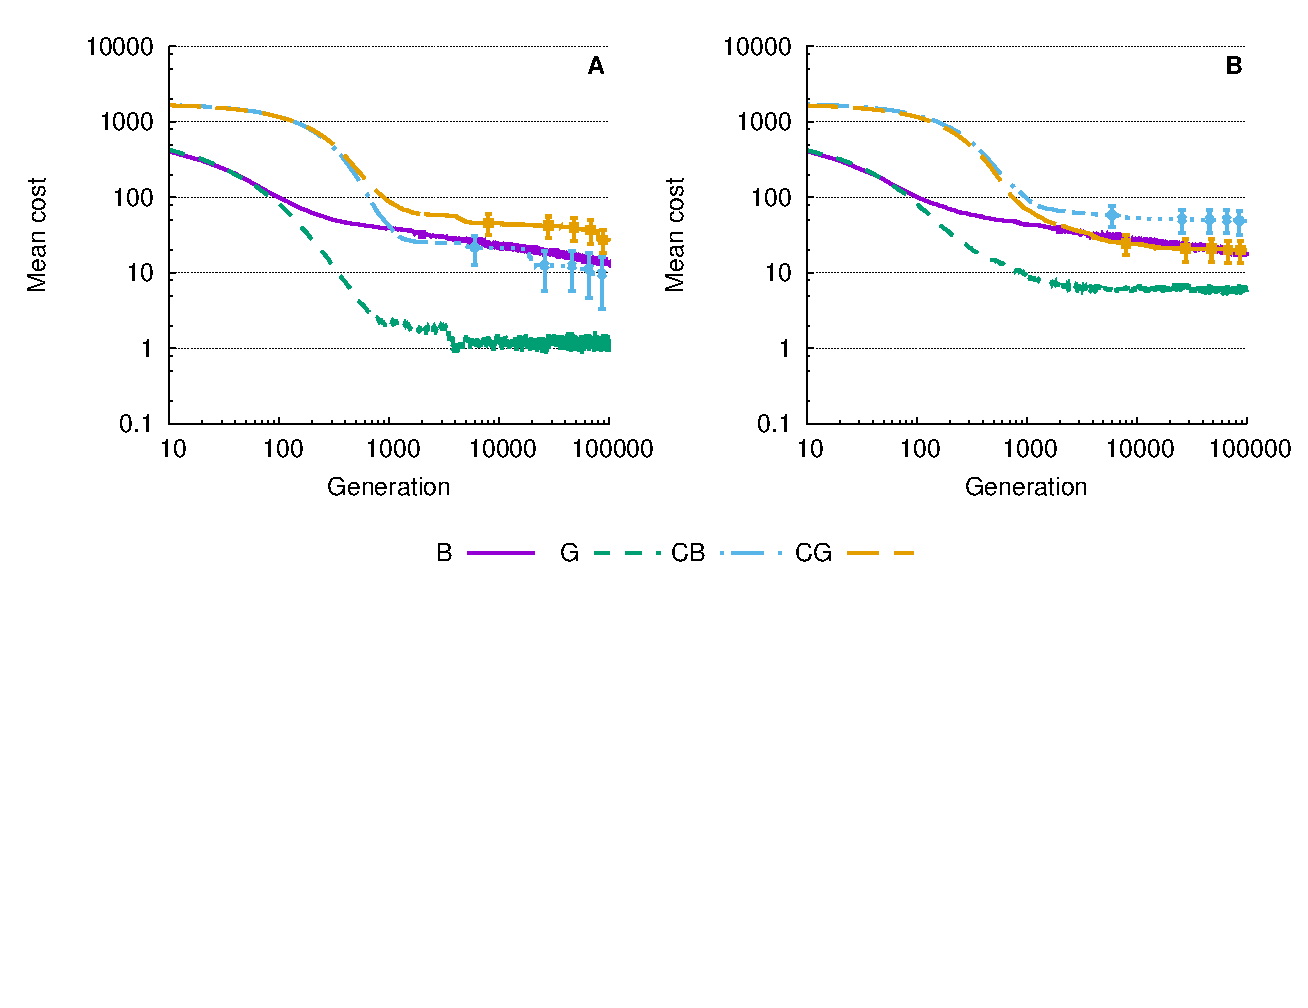
\includegraphics[trim=0 4cm 0 0,scale=.5]{multievola-b}
   \end{figure}
   \vspace{-3.5cm}
      \textbf{A:\ Linear, B:\ Stairs}
   \begin{itemize}
      \item Gray code performs the best. Binary is grouped with consensus
         encodings.
      \item Binary performance is unaffected by complexity changes
   \end{itemize}
\end{frame}
\begin{frame}
   \frametitle{Performance}
   \vspace{2.5cm}
   \begin{figure}[H]
      \centering
      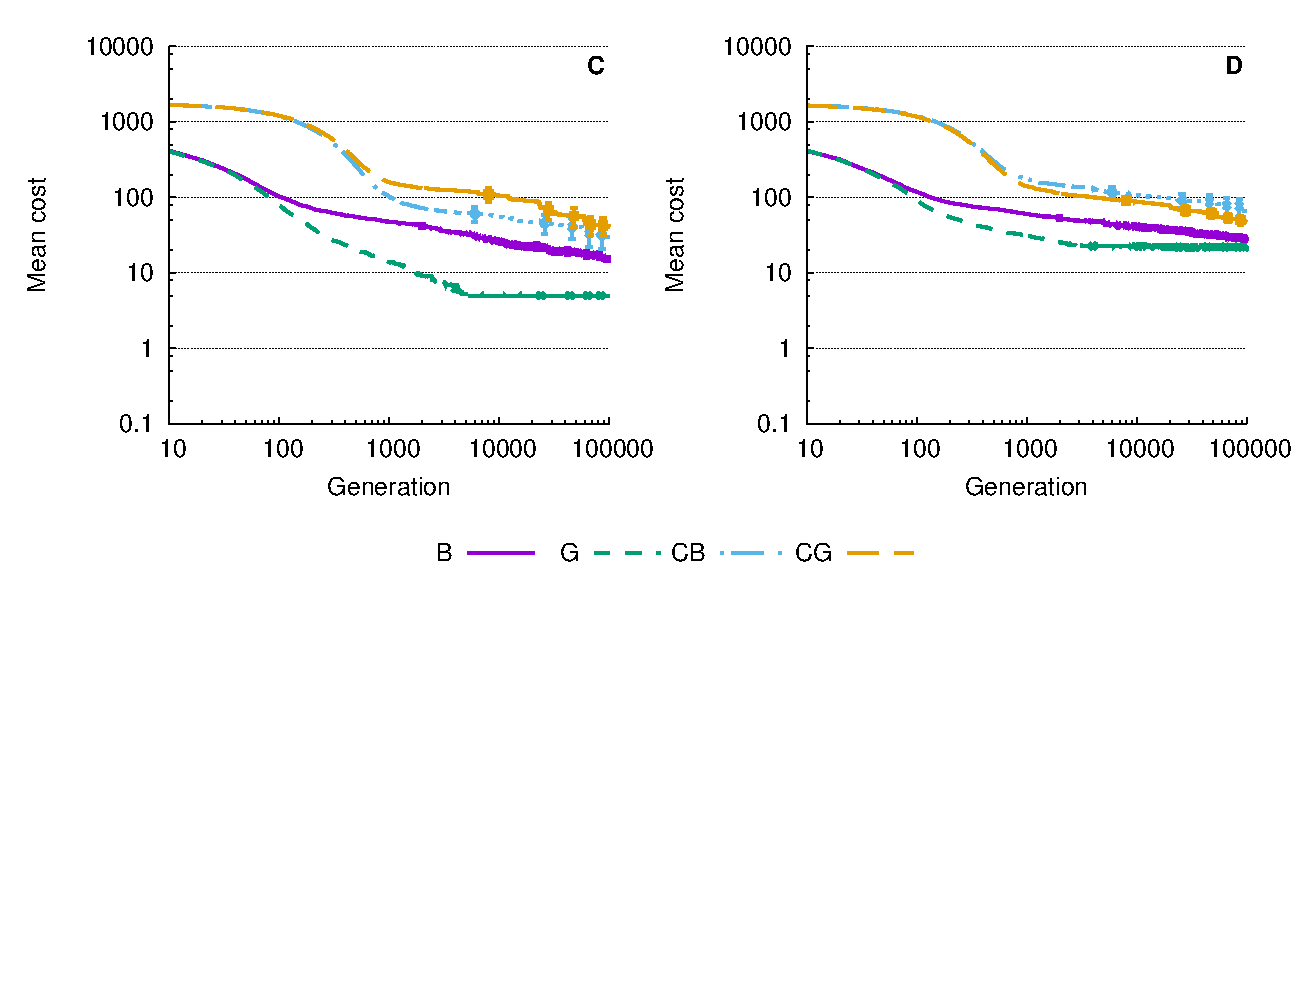
\includegraphics[trim=0 4cm 0 0,scale=.5]{multievolc-d}
   \end{figure}
   \vspace{-3.5cm}
      \textbf{C:\ Moguls, D:\ Sharktooth}
   \begin{itemize}
      \item With high enough complexity, Gray code loses its benefits
   \end{itemize}
\end{frame}

\begin{frame}
   \frametitle{Distribution of cost effects -- Linear transformation}
   \vspace{2cm}
   \hspace{-4cm}~\begin{figure}
      \hspace{-4.5em}
      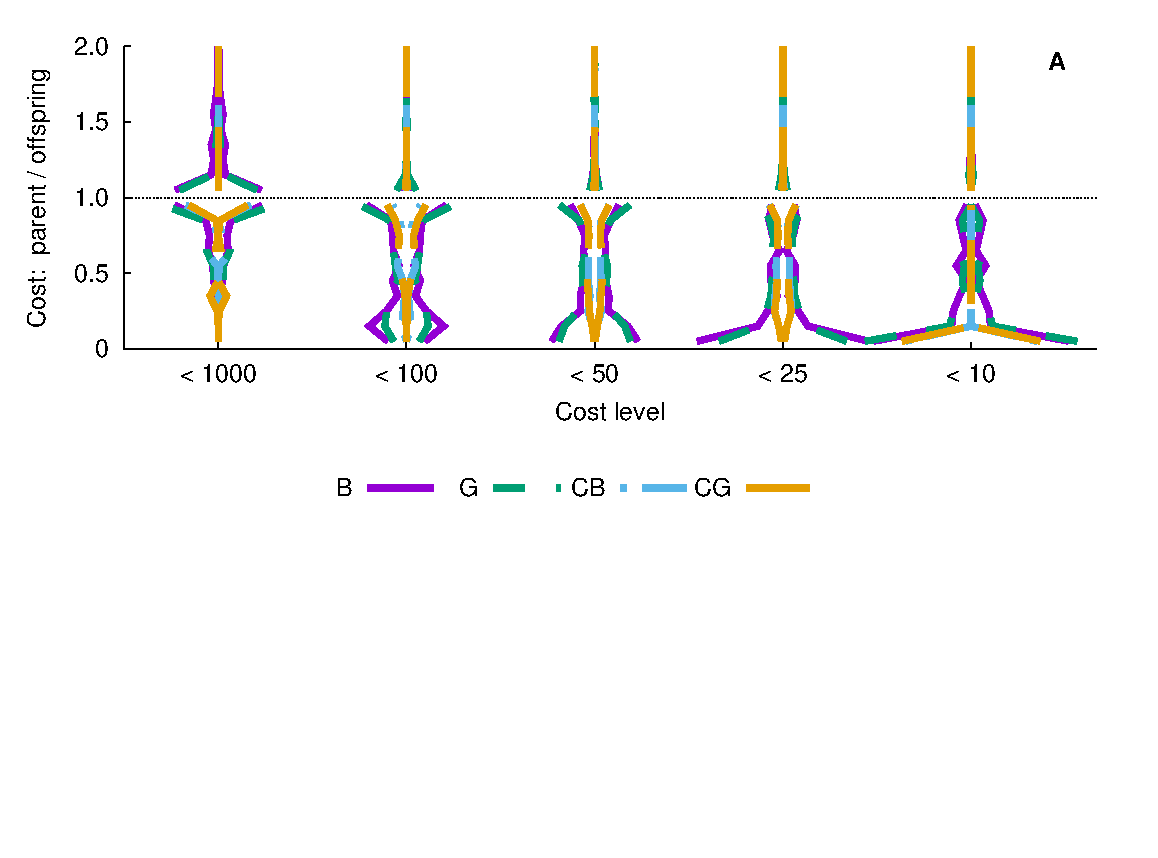
\includegraphics[trim=0 4cm 0 0,scale=.65]{linear_histo}
      \hspace{-4em}
   \end{figure}
   \vspace{-4cm}
   \begin{itemize}
      \item Binary and Gray are similar. Consensus encodings are similar.
      \item Gray code has consistent positive mutations
      \item Consensus encodings evolve by adding and removing random numbers
   \end{itemize}
\end{frame}

\begin{frame}
   \frametitle{Robustness -- Linear transformation}
   \vspace{3cm}
   \begin{figure}
      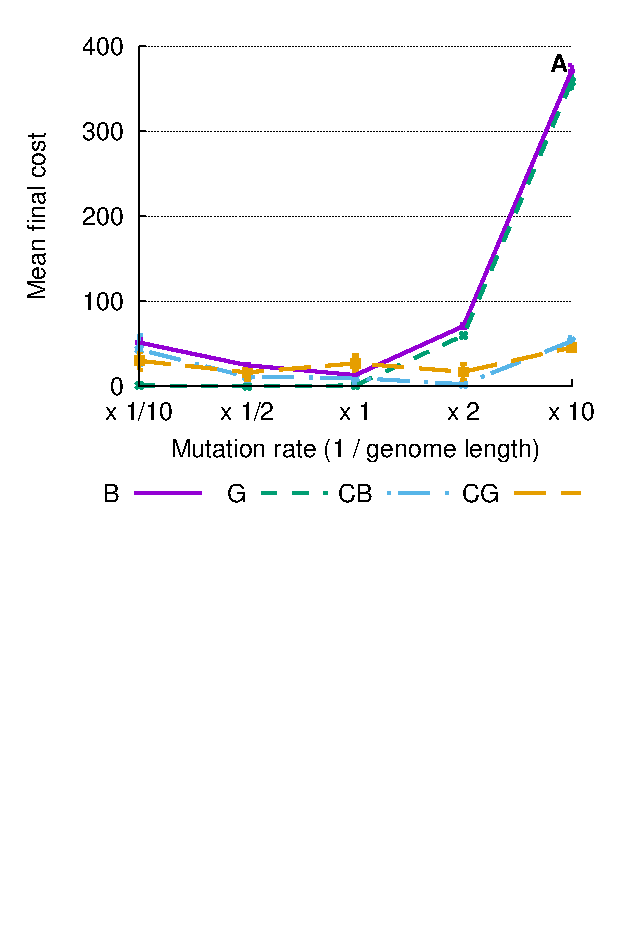
\includegraphics[trim=0 4.2cm 0 0,scale=.7]{pres_mutrates_a}
   \end{figure}
   \vspace{-5cm}
   \begin{itemize}
      \item Consensus encodings are more robust, bijective encodings sensitive
            to high mutation rates
      \item Gray code evolves mainly by single bit flips, Binary by multiple
   \end{itemize}
\end{frame}
\section{Concluding remarks}
\begin{frame}
   \frametitle{Implication of the results}
   \begin{itemize}
      \item The different modes of evolution give rise to different overall
         evolutionary dynamics
      \item Bijectivity is not everything -- also directly available states and
      the connectivity between states matter
      \item Non-bijectivity make for more flexible genomes
   \end{itemize}
\end{frame}



\begin{frame}[standout]
      Thank you!
   \end{frame}

\begin{frame}
   \thispagestyle{empty}
\end{frame}

   \begin{frame}
      \frametitle{Binary--Gray code table}
      \begin{table}
         \centering
         \begin{tabular}{cccc}
            \toprule
            \textbf{Integer} & \textbf{Binary} & \textbf{Gray} &
            \textbf{Gray as integer} \\
            \midrule
            0 & 000 &  000 &  0 \\  
            1 & 001 &  001 &  1 \\
            2 & 010 &  011 &  3 \\
            3 & 011 &  010 &  2 \\
            4 & 100 &  110 &  6 \\
            5 & 101 &  111 &  7 \\
            6 & 110 &  101 &  5 \\
            7 & 111 &  100 &  4 \\
            \bottomrule
         \end{tabular}
      \end{table}
   \end{frame}


   \begin{frame}
      \frametitle{What about the biology?}
      \begin{itemize}
         \item Biological genetic strands carry large amounts of "dead code"
         \item Natural evolution is a product of itself -- what are the alternatives?
         \item Evolutionary mechanisms are complex and not well understood
      \end{itemize}
   \end{frame}
\begin{frame}
   \frametitle{Distribution of cost effects -- Stairs transformation}
   \vspace{2.5cm}
   \hspace{-4cm}~\begin{figure}
      \hspace{-4.5em}
      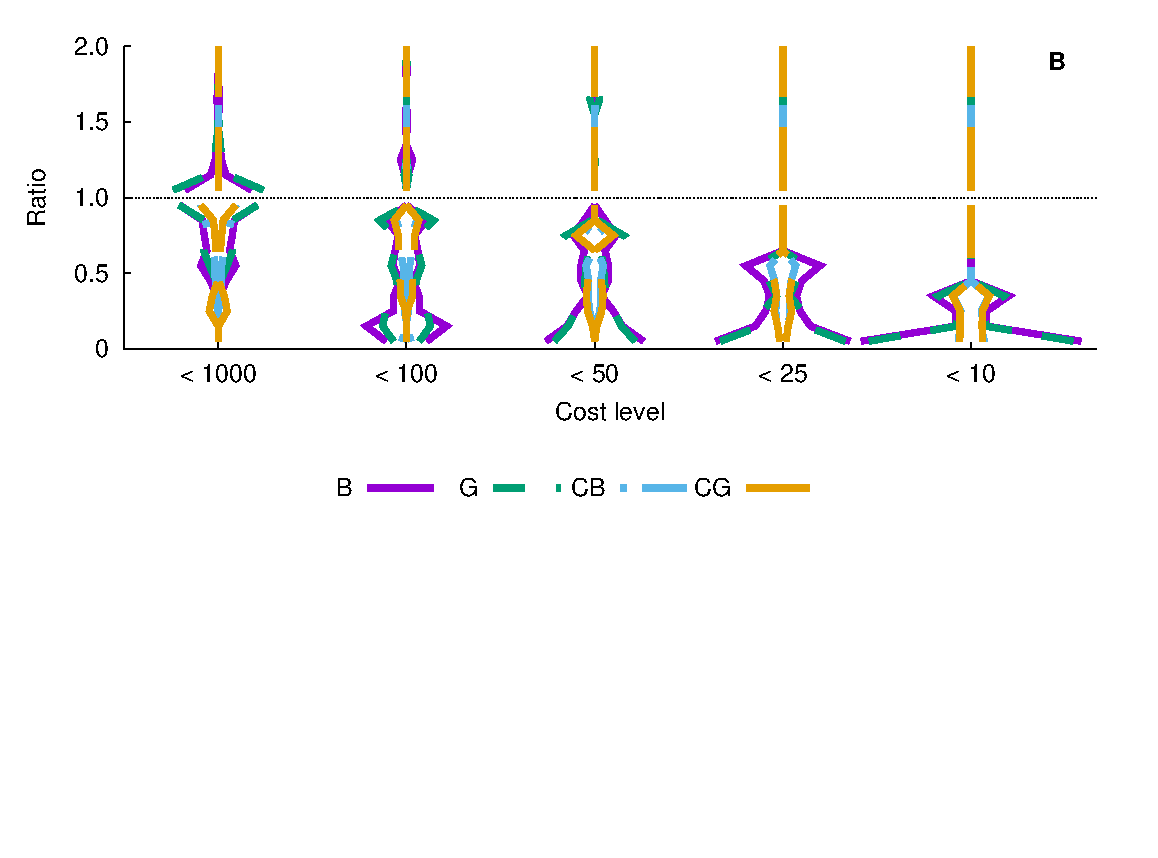
\includegraphics[trim=0 3cm 0 0,scale=.65]{ladder_histo}
      \hspace{-4em}
   \end{figure}
   \vspace{-3.5cm}
\end{frame}
\begin{frame}
   \frametitle{Distribution of cost effects -- Moguls transformation}
   \vspace{2.5cm}
   \hspace{-4cm}~\begin{figure}
      \hspace{-4.5em}
      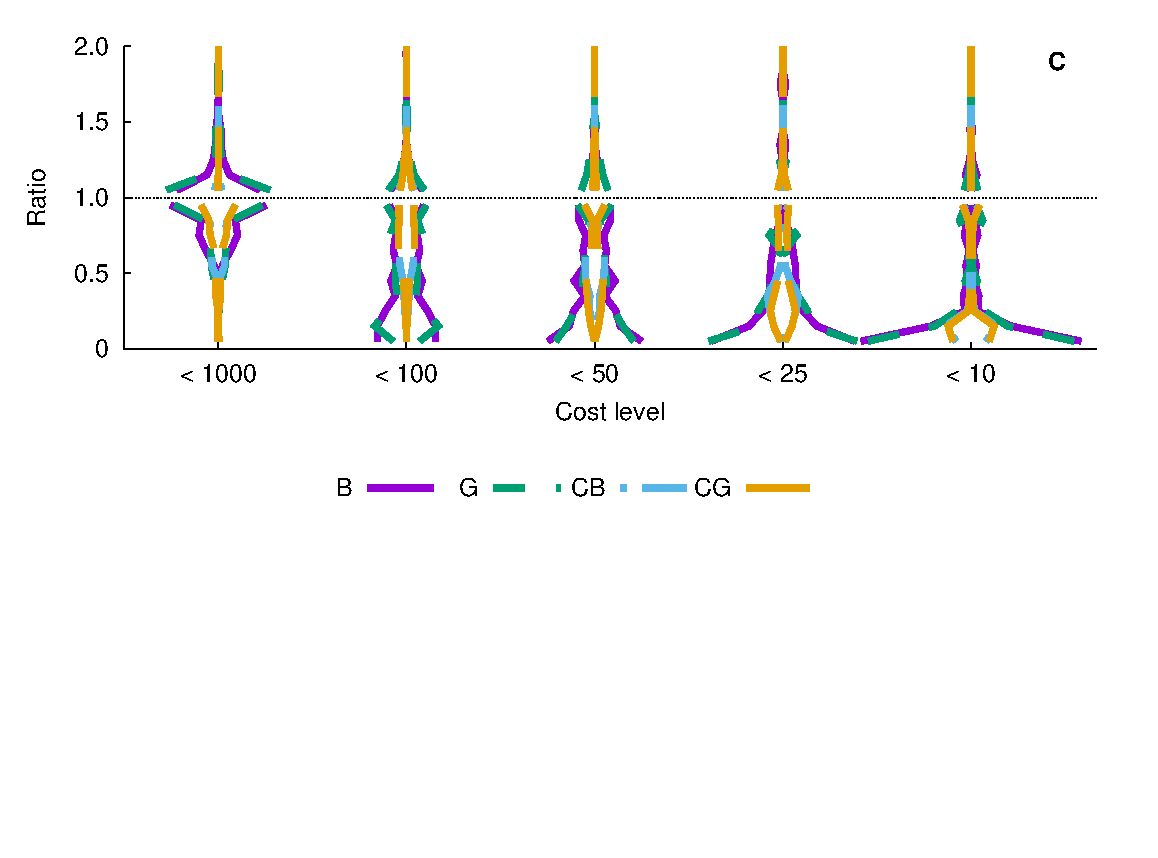
\includegraphics[trim=0 4cm 0 0,scale=.65]{sinusoidal_histo}
      \hspace{-4em}
   \end{figure}
   \vspace{-3.5cm}
\end{frame}
\begin{frame}
   \frametitle{Distribution of cost effects -- Sharktooth transformation}
   \vspace{2.5cm}
   \hspace{-4cm}~\begin{figure}
      \hspace{-4.5em}
      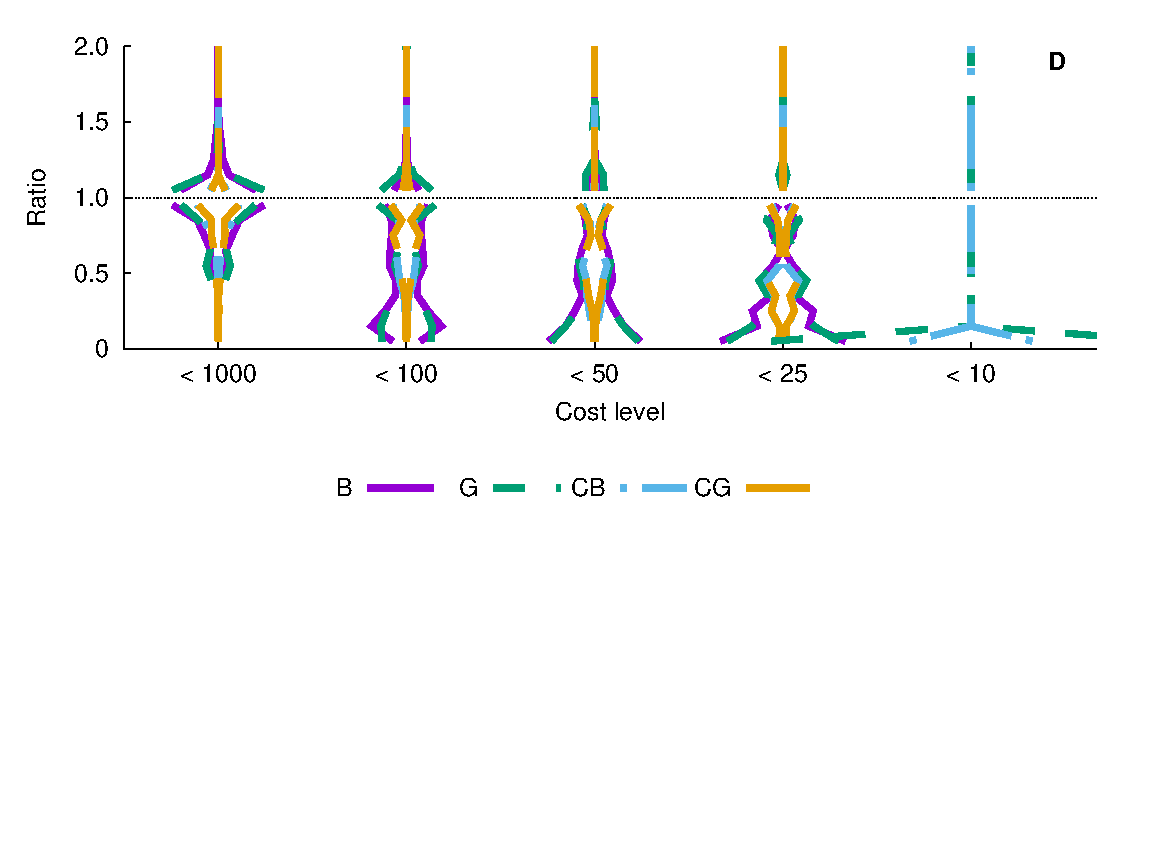
\includegraphics[trim=0 4cm 0 0,scale=.65]{hard_sinusoidal_histo}
      \hspace{-4em}
   \end{figure}
   \vspace{-3.5cm}
\end{frame}
\begin{frame}
   \frametitle{Robustness -- Stairs transformation}
   \vspace{3cm}
   \begin{figure}
      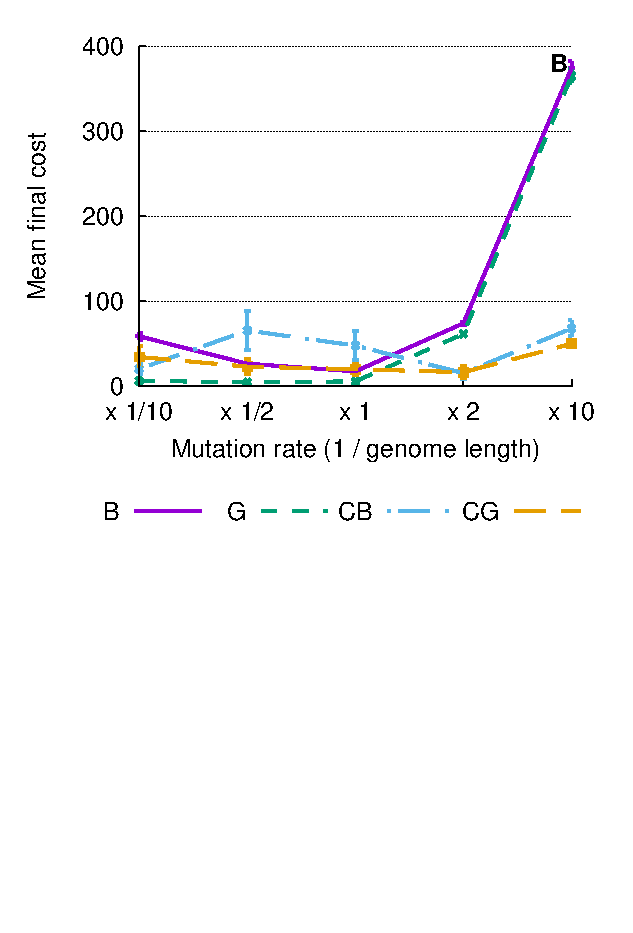
\includegraphics[trim=0 4.2cm 0 0,scale=.7]{pres_mutrates_b}
   \end{figure}
   \vspace{-4.5cm}
\end{frame}
\begin{frame}
   \frametitle{Robustness -- Moguls transformation}
   \vspace{3cm}
   \begin{figure}
      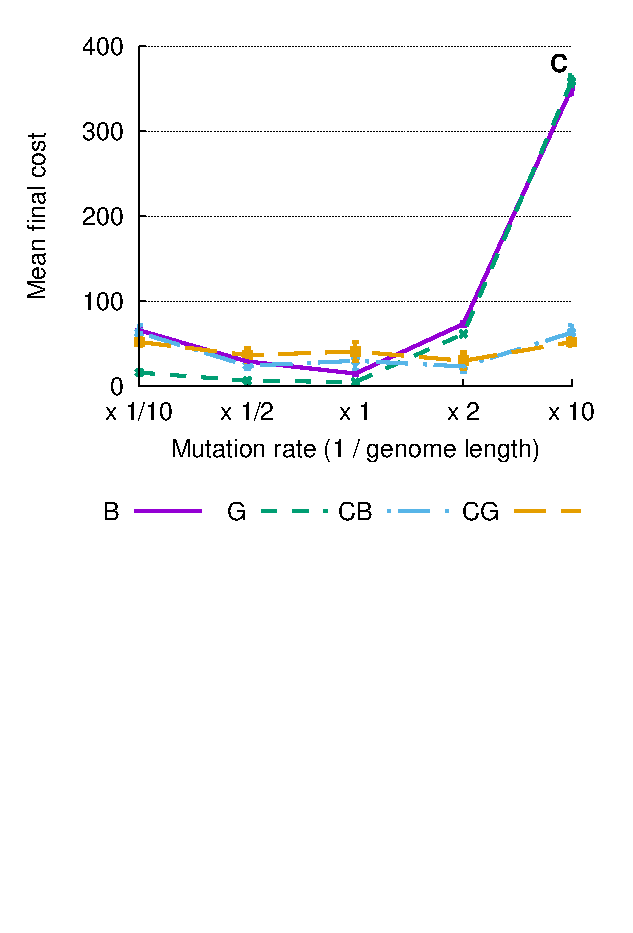
\includegraphics[trim=0 4.2cm 0 0,scale=.7]{pres_mutrates_c}
   \end{figure}
   \vspace{-4.5cm}
\end{frame}
\begin{frame}
   \frametitle{Robustness -- Sharktooth transformation}
   \vspace{3cm}
   \begin{figure}
      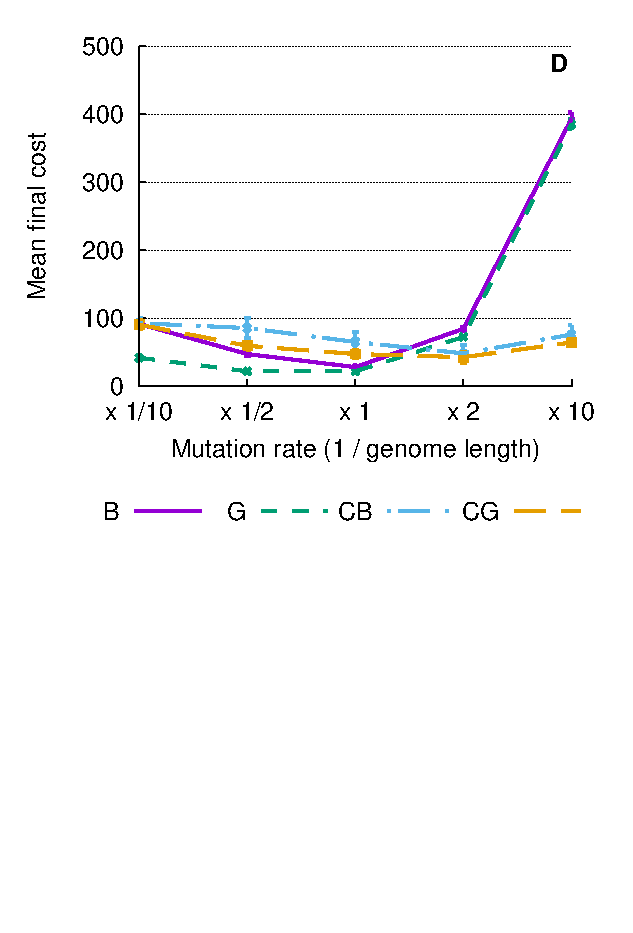
\includegraphics[trim=0 4.2cm 0 0,scale=.7]{pres_mutrates_d}
   \end{figure}
   \vspace{-4.5cm}
\end{frame}
\end{document}
